\section{System}\label{sec:system}

\acde{} is organised in three planes (Figure~\ref{fig:arch} summarises the flow).

\begin{figure}[t]
\centering
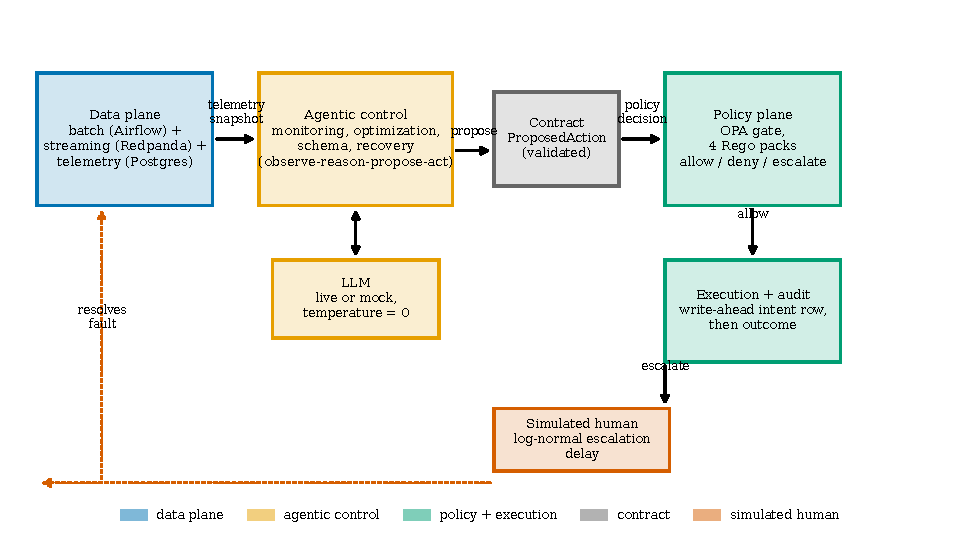
\includegraphics[width=0.95\linewidth]{generated/fig_arch.pdf}
\caption{System overview: a telemetry snapshot from the data plane drives the agentic control loop
  (observe--reason--propose--act, live or mock model); every proposal is validated against the
  \texttt{ProposedAction} contract before the policy plane's OPA gate allows, denies, or escalates it;
  an allowed action is executed under a write-ahead audit trail; an escalated one resolves through the
  simulated human's log-normal delay, whose resolution is what closes an open fault back in the data
  plane (dotted path).}
\label{fig:arch}
\end{figure}

\paragraph{Data plane.}
A batch pipeline in Apache Airflow ingests a TPC-DS-derived dataset into versioned warehouse
partitions; a streaming consumer reads from a Redpanda topic; all telemetry (pipeline metrics,
resource usage, task runs, agent actions, failure events, manual interventions) is written to a
PostgreSQL \texttt{telemetry} schema from which every experimental metric is reconstructed.

\paragraph{Agentic control plane.}
Four agents share one loop: \emph{observe} a telemetry snapshot, \emph{reason} (a live or mock
language model), \emph{propose}, \emph{act}. The monitoring agent is the detector and is enabled in
every non-baseline configuration so that recovery time is measurable; optimisation scales workers or
pool slots or reprioritises; the schema agent allows compatible changes or contains breaking ones;
the recovery agent retries, replays, rolls back, recomputes partially, or escalates to a human.
Same-target proposals are resolved by a static agent-priority bid.

\paragraph{The contract.}
An agent's only output is a \texttt{ProposedAction}: agent, action type, target, parameters,
justification, confidence. It is validated by a typed schema (pydantic) that rejects any action type
outside the agent's allowlist and, since this work, any scaling target that is not an integer
$\geq 1$. Invalid output is rejected, logged, and counted as \texttt{agent\_output\_invalid}; it
degrades to \texttt{no\_action}. Agents never emit or execute code.

\paragraph{Policy plane.}
Each proposal, with a system-built context (projected marginal cost, remaining budget, actions in
the last ten minutes, schema compatibility, prior-version existence), is evaluated by four Rego
policy packs: a rate limit (at most four actions per agent per ten minutes), a cost budget, a
recovery-approval policy (rollback only with a prior version), and a schema-compatibility policy.
The decision is one of allow, deny, escalate, or allow-and-notify. If the policy engine is
unreachable the gate escalates; it never allows.

\paragraph{Execution and audit.}
An intent row is written and committed \emph{before} the executor runs (a write-ahead audit trail),
then updated with the outcome; a crash mid-action leaves a durable \texttt{executing} row.

\paragraph{Simulated human.}
Escalations resolve after a seeded log-normal delay (median \NHumanMedian{}\,s, $\sigma=\NHumanSigma{}$):
the simulated on-call. This is a modelling choice, not a measurement, and \S\ref{sec:results}
quantifies how much the headline results depend on it.
